\documentclass{article}

\usepackage[utf8]{inputenc}
\usepackage{amsthm}
\usepackage{amssymb}
\usepackage{mathtools}
\usepackage{graphicx}
\usepackage{mdframed}
\usepackage{float}
\usepackage[top=0.75in, bottom=0.75in, left=0.75in, right=0.75in]{geometry}
\usepackage{gauss}

\usepackage{array}
\allowdisplaybreaks

\makeatletter
\newcounter{elimination@steps}
\newcolumntype{R}[1]{>{\raggedleft\arraybackslash$}p{#1}<{$}}
\def\elimination@num@rights{}
\def\elimination@num@variables{}
\def\elimination@col@width{}
\newenvironment{elimination}[4][0]
{
    \setcounter{elimination@steps}{0}
    \def\elimination@num@rights{#1}
    \def\elimination@num@variables{#2}
    \def\elimination@col@width{#3}
    \renewcommand{\arraystretch}{#4}
    \start@align\@ne\st@rredtrue\m@ne
}
{
    \endalign
    \ignorespacesafterend
}
\newcommand{\step}[2]
{
    \ifnum\value{elimination@steps}>0\sim\quad\fi
    \left[
        \ifnum\elimination@num@rights>0
            \begin{array}
            {@{}*{\elimination@num@variables}{R{\elimination@col@width}}
            |@{}*{\elimination@num@rights}{R{\elimination@col@width}}}
        \else
            \begin{array}
            {@{}*{\elimination@num@variables}{R{\elimination@col@width}}}
        \fi
            #1
        \end{array}
    \right]
    & 
    \begin{array}{l}
        #2
    \end{array}
    \addtocounter{elimination@steps}{1}
}
\makeatother

\DeclarePairedDelimiter{\abs}{\lvert}{\rvert}
\DeclarePairedDelimiter{\norm}{\lvert \lvert}{\rvert \rvert}

\newtheoremstyle{break}% name
  {}%         Space above, empty = `usual value'
  {}%         Space below
  {\itshape}% Body font
  {}%         Indent amount (empty = no indent, \parindent = para indent)
  {\bfseries}% Thm head font
  {.}%        Punctuation after thm head
  {\newline}% Space after thm head: \newline = linebreak
  {}%         Thm head spec

\newtheorem{Def}{Definition}[section]

\theoremstyle{break}

\newtheorem{innerEx}{Exempel}[section]
\newtheorem{sats}{Sats}[section]
\newtheorem{Rem}{Anmärkning}[]

\newenvironment{Ex}
{\begin{mdframed} \begin{innerEx} \vspace{3pt}}
{\vspace{3pt} \end{innerEx} \end{mdframed}}  

\newenvironment{bevis}
{\begin{mdframed} \begin{proof} \vspace{3pt}}
{\vspace{3pt} \end{proof} \end{mdframed}}

\title{
	 Linjär Algebra\\
	 Föreläsning 7
    \author{Erik Sjöström}
}
\begin{document}
\maketitle

\section{Avbildningar} % (fold)
\label{sec:avbildningnar}
En avbildning:
\[
f: \mathbb{R}^n \rightarrow \mathbb{R}^m
\]
är en regel som till varje vektor $\vec{x} \in \mathbb{R}^n$ ordnar en vektor $f(\vec{x}) \in \mathbb{R}^n$ 
\begin{itemize}
	\item $\mathbb{R}^n$ kallas för definitionsmängd (alla tillåtna $\vec{x}$)
	\item $\mathbb{R}^m$ kallas för målmängd
	\item För ett givet $\vec{x}$ kallas $f(\vec{x})$ för \underline{bilden} av $\vec{x}$ (under avbildningen $f$)
\end{itemize}
\begin{Ex}
    Låt $f(x) = 3 \cdot x$ vara avbildningen $\mathbb{R} \rightarrow \mathbb{R}$\\
    Bilden av $x = \frac{5}{3}$ är 5 ty $f(\vec{x}) = 3 \cdot \frac{5}{3} = 5$
\end{Ex}
\begin{Ex}
    Låt:
    \begin{align*}
    &A= \begin{bmatrix} 1&1\\1&-1 \end{bmatrix}, &&f(\vec{x}) = A \cdot \vec{x} \mbox{,  }\mbox{ }\mbox{ }\forall \vec{x} \in \mathbb{R}^2
    \end{align*}
    Dvs:
    \[
        f(\vec{x}) = \begin{bmatrix} 1&1\\1&-1 \end{bmatrix} \cdot \begin{bmatrix} x\\y \end{bmatrix} = \begin{bmatrix} x+y\\x-y \end{bmatrix}
    \]
    Bilden av $\begin{bmatrix} 3\\5 \end{bmatrix}$ är $\begin{bmatrix} 8\\-2 \end{bmatrix}$ ty:
    \[
        f(\begin{bmatrix} 3\\5 \end{bmatrix}) = \begin{bmatrix} 1&1\\1&-1 \end{bmatrix} \cdot \begin{bmatrix} 3\\5 \end{bmatrix} = \begin{bmatrix} 3+5\\3-5 \end{bmatrix} = \begin{bmatrix} 8\\-2 \end{bmatrix}
    \]
    Vi har alltså en avbildning:
	\[
	    f: \mathbb{R}^2 \rightarrow \mathbb{R}^2
	\]
\end{Ex}
\newpage
\begin{Def}
    En avbildning $f: \mathbb{R}^n \rightarrow \mathbb{R}^m$ är \underline{linjär} om:
    \begin{itemize}
    	\item $f(\vec{u} + \vec{v}) = f(\vec{u}) + f(\vec{v})$
    	\item $f(c \cdot \vec{u}) = c \cdot f(\vec{u})$
    \end{itemize}
    $\forall \vec{u}, \vec{v} \in \mathbb{R}^n$ och $c \in \mathbb{R}$
\end{Def}
\begin{sats}
    Låt $f: \mathbb{R}^n \rightarrow \mathbb{R}^m$ och låt $f(\vec{x}) = A \cdot \vec{x}$, då är $f$ en linjär avbildning.
\end{sats}
\noindent
Visas genom att visa att matrisvektorprodukten uppfyller villkoren för en linjär avbildning.
\begin{bevis}
Låt $\vec{x}_1$ och $\vec{x}_2$ vara två stycken $(n \times 1)$ vektorer, vi har då:
	\begin{itemize}
		\item $f(\vec{x}_1 + \vec{x}_2) = A \cdot (\vec{x}_1 + \vec{x}_2) = A \cdot \vec{x}_1 + A \cdot \vec{x}_2 = f(\vec{x}_1) + f(\vec{x}_2)$
		\item $f(c \cdot \vec{x}_1) = A \cdot (c \cdot \vec{x}_1) = (c \cdot A) \cdot \vec{x}_1 = c \cdot (A \cdot \vec{x}_1) = c \cdot f(\vec{x}_1)$
	\end{itemize}
\end{bevis}
\begin{sats}[Bassatsen]
    Låt $f: \mathbb{R}^n \rightarrow \mathbb{R}^m$ vara en linjär avbildning. Då finns det en entydigt bestämd matris $A_{m \times n}$ sådan att $f(\vec{x}) = A \cdot \vec{x}$
\end{sats}
\begin{bevis}
	i $\mathbb{R}^2$\\
	Varje vektor $\vec{x} = \begin{bmatrix} x\\y \end{bmatrix}$ kan skrivas som en linjärkombination av basvektorerna:
	\[
	   \vec{x} = x \cdot \vec{e}_x + y \cdot \vec{e}_y = x \cdot \begin{bmatrix} 1\\0 \end{bmatrix} + y \cdot \begin{bmatrix} 0\\1 \end{bmatrix}
	 \]
	 Vi har då:
	 \[
	     f(\vec{x}) = f(x \cdot \vec{e}_x + y \cdot \vec{e}_y) = x \cdot f(\vec{e}_x) + y \cdot f(\vec{e}_y) = \overbrace{\begin{bmatrix} f(\vec{e}_x)&f(\vec{e}_y) \end{bmatrix}}^\text{$A$ = Standardmatrisen} \cdot \begin{bmatrix} x\\y \end{bmatrix}
	 \]
	 Avbildningen bestäms helt av vad den gör med $\vec{e}_x$ och $\vec{e}_y$. 
\end{bevis}

\begin{Ex}
    Låt $f(\vec{x}) = \begin{bmatrix} x+y\\x-y \end{bmatrix}$ vara avbildningen $\mathbb{R}^2\rightarrow \mathbb{R}^2$. Bestäm standardmatrisen $A$.\\
    \textbf{Lösning:} Eftersom:
    \begin{align*}
    &\vec{e}_x = \begin{bmatrix} 1\\0 \end{bmatrix} &\vec{e}_y = \begin{bmatrix} 0\\1 \end{bmatrix}
    \end{align*}
    får vi:
    \begin{gather}
    	f(\vec{e}_x) = f(\begin{bmatrix} 1\\0 \end{bmatrix}) = \begin{bmatrix} 1+0\\1-0 \end{bmatrix} = \begin{bmatrix} 1\\1 \end{bmatrix} \\
    	f(\vec{e}_y) = f(\begin{bmatrix} 0\\1 \end{bmatrix}) = \begin{bmatrix} 0+1\\0-1 \end{bmatrix} = \begin{bmatrix} 1\\-1 \end{bmatrix}
    \end{gather}
    Vi får då standardmatrisen:
    \[
        A = \begin{bmatrix} 1&1\\1&-1 \end{bmatrix}
    \]
\end{Ex}

\begin{Ex}
	Låt $f: \mathbb{R}^2 \rightarrow \mathbb{R}^2$ vara rotationen moturs med vinkeln $\theta$. Bestäm standardmatrisen $A$.
	\begin{center}
		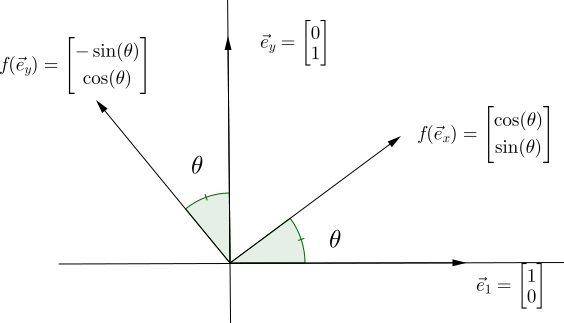
\includegraphics[scale=0.5]{roation.png}	    	
	\end{center}	
	\begin{align*}
	&f(\vec{e}_x) = f(\begin{bmatrix} 1\\0 \end{bmatrix}) = \begin{bmatrix} \cos(\theta)\\\sin(\theta) \end{bmatrix} && &&&f(\vec{e}_y) = f(\begin{bmatrix} 0\\1 \end{bmatrix}) = \begin{bmatrix} -\sin(\theta)\\\cos(\theta) \end{bmatrix}\\
	&&A = \begin{bmatrix} \cos(\theta)&-\sin(\theta)\\\sin(\theta)&\cos(\theta) \end{bmatrix}
	\end{align*}
	Kallas även rotationsmatrisen.
\end{Ex}
\newpage
\noindent
Låt $f: \mathbb{R}^n \rightarrow \mathbb{R}^m$ vara en linjär avbildning och $f(\vec{x}) = A \cdot \vec{x}$. Bilden av en linje $L$ där:
\[
    L: \vec{x}_0 + t \cdot \vec{v}
\]
$t\in \mathbb{R}$\\
Blir en linje som går genom en punkt $A \cdot \vec{x}_0$ med riktningsvektor $A \cdot \vec{v}$, ty:
\[
    f(\vec{x}_0 + t \cdot \vec{v}) = f(\vec{x}_0) + t \cdot f(\vec{v}) = A \cdot \vec{x}_0 + t \cdot A \cdot \vec{v}
\]
Följden blir att vi kan avbilda n-hörningar.
\begin{Ex}
    Rotera ett område vars hörn består av:
    \begin{align*}
    &\vec{x}_1 = \begin{bmatrix} 1\\1 \end{bmatrix}
    &&&\vec{x}_2 = \begin{bmatrix} 3\\3 \end{bmatrix}
    &&&&\vec{x}_3 = \begin{bmatrix} 4\\3 \end{bmatrix}
    &&&&&\vec{x}_4 = \begin{bmatrix} 2\\1 \end{bmatrix}
    \end{align*}
    $\pi/6$ radianer moturs.
    \begin{align*}
    	A &= \begin{bmatrix} cos(\pi/6)&-sin(\pi/6)\\sin(\pi/6)&cos(\pi/6)\end{bmatrix} = \begin{bmatrix} \sqrt{3}/2&-1/2\\1/2&\sqrt{3}/2 \end{bmatrix}\\
    	A \cdot \vec{x}_1 &= \begin{bmatrix} cos(\pi/6)&-sin(\pi/6)\\sin(\pi/6)&cos(\pi/6)\end{bmatrix} = \begin{bmatrix} \sqrt{3}/2&-1/2\\1/2&\sqrt{3}/2 \end{bmatrix} \begin{bmatrix} 1\\1 \end{bmatrix} = \begin{bmatrix} \sqrt{3}/2-1/2\\1/2+\sqrt{3}/2 \end{bmatrix}\\
    	A \cdot \vec{x}_2 &= \cdots \\
    	A \cdot \vec{x}_3 &= \cdots\\
    	A \cdot \vec{x}_4 &= \cdots
    \end{align*}
    \begin{center}
    	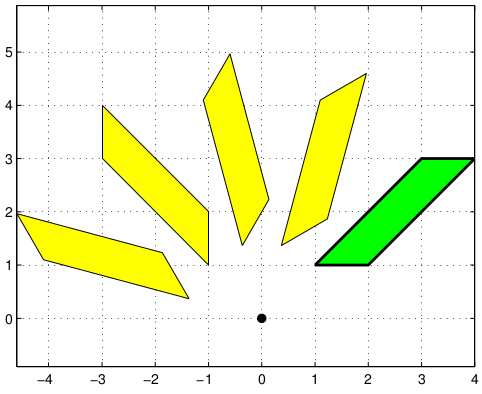
\includegraphics[scale=0.5]{F7.png}
    \end{center}
\end{Ex}
Translation (förflyttning) med vektor $t = \begin{bmatrix} t_1\\t_2 \end{bmatrix}$ ges av avbildningen:
\begin{gather*}
	f: \mathbb{R}^2 \rightarrow \mathbb{R}^2\\
	f(\vec{x}) = \vec{x} + \vec{t} = \begin{bmatrix} x\\y \end{bmatrix} + \begin{bmatrix} t_1\\t_2 \end{bmatrix}
\end{gather*}
Är avbildningen linjär?\\
Låt $\vec{u}, \vec{v} \in \mathbb{R}^2$
\[
    f(\vec{u} + \vec{v}) = (\vec{u} + \vec{v}) + \vec{t} \neq f(\vec{u}) + f(\vec{v})
\]
Den är ej linjär, så det finns ingen \underline{standardmatris}. Men vi kan såklart fortfarande räkna på det.
\begin{Ex}
    Translatera området vars hörn består av:
    \begin{align*}
    &\vec{x}_1 = \begin{bmatrix} 1\\1 \end{bmatrix}
    &&&\vec{x}_2 = \begin{bmatrix} 3\\3 \end{bmatrix}
    &&&&\vec{x}_3 = \begin{bmatrix} 4\\3 \end{bmatrix}
    &&&&&\vec{x}_4 = \begin{bmatrix} 2\\1 \end{bmatrix}
    \end{align*}
    Låt $\vec{t} = \begin{bmatrix} 0\\3 \end{bmatrix}$
    \begin{gather*}
    	f(x_1) = f(\begin{bmatrix} 1\\1 \end{bmatrix}) = \begin{bmatrix} 1\\1 \end{bmatrix} + \begin{bmatrix} 0\\3 \end{bmatrix} = \begin{bmatrix} 1\\4 \end{bmatrix}\\
    	f(x_2) = f(\begin{bmatrix} 3\\3 \end{bmatrix}) = \begin{bmatrix} 3\\3 \end{bmatrix} + \begin{bmatrix} 0\\3 \end{bmatrix} = \begin{bmatrix} 3\\6 \end{bmatrix}
    \end{gather*}
    \begin{center}
    	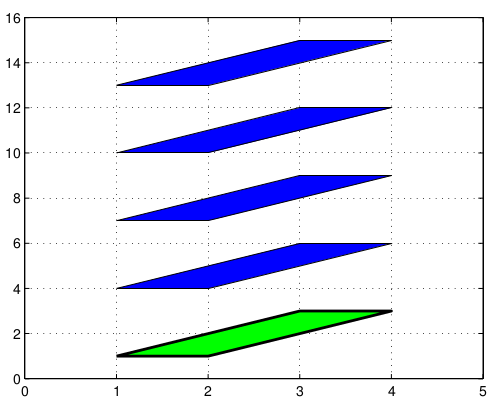
\includegraphics[scale=0.5]{F7plan.png}
    \end{center}
\end{Ex}
\section{Rotation och translation i $\mathbf{\mathbb{R}^3}$} % (fold)
\label{sec:rotation_och_translation_i_}
Går till på samma sätt som i $\mathbb{R}^2$
\begin{Ex}
    Rotation moturs $\theta$ i radianer i xy-planet
    \[
        A = \begin{bmatrix} \cos(\theta)&-\sin(\theta)\\\sin(\theta)&\cos(\theta) \end{bmatrix}
    \]
    Låt $f: \mathbb{R}^3 \rightarrow \mathbb{R}^3$ vara:
    \begin{align*}
    &f(\vec{e}_x) = \begin{bmatrix} \cos(\theta)\\\sin(\theta)\\0 \end{bmatrix}
    &&f(\vec{e}_y) = \begin{bmatrix} -\sin(\theta)\\\cos(\theta)\\0 \end{bmatrix}
    &&&f(\vec{e}_z) = \begin{bmatrix} 0\\0\\1 \end{bmatrix}
    \end{align*}
    $\Rightarrow$ Standardmatris:
    \[
        A = \begin{bmatrix} \cos(\theta)&-\sin(\theta)&0\\\sin(\theta)&\cos(\theta)&0\\0&0&1 \end{bmatrix}
    \]
    Vilket då blir en rota ion moturs runt Z-axeln.
\end{Ex}

% section rotation_och_translation_i_ (end)
% section avbildningnar (end)

\end{document}
